\documentclass[conference]{IEEEtran}
\IEEEoverridecommandlockouts
% The preceding line is only needed to identify funding in the first footnote. If that is unneeded, please comment it out.
%\usepackage{cite}
\usepackage{amsmath,amssymb,amsfonts}
\usepackage{algorithmic}
\usepackage{graphicx}
\usepackage{textcomp}
\usepackage{xcolor}
\usepackage{float}

\usepackage{tikz}
\usetikzlibrary{arrows,shadows,trees,shapes,decorations,automata,backgrounds,petri,mindmap} % for pgf-umlsd
\usepackage[oldvoltagedirection,american,cuteinductors,smartlabels]{circuitikz}
\usetikzlibrary{calc}
\ctikzset{bipoles/thickness=1}
\ctikzset{bipoles/length=0.8cm}
\ctikzset{bipoles/diode/height=.375}
\ctikzset{bipoles/diode/width=.3}
\ctikzset{tripoles/thyristor/height=.8}
\ctikzset{tripoles/thyristor/width=1}
\ctikzset{bipoles/vsourceam/height/.initial=.7}
\ctikzset{bipoles/vsourceam/width/.initial=.7}
\tikzstyle{every node}=[font=\small]
\tikzstyle{every path}=[line width=0.8pt,line cap=round,line join=round]
\usetikzlibrary{fit,positioning,shapes.geometric}

%Biber using IEEE style for proper UTF-8 support
\usepackage[backend=biber,style=ieee, sorting=none, maxnames=1,minnames=1]{biblatex}
\bibliography{bib/myrefs}

\usepackage{csquotes}

\usepackage{stfloats}

%\def\BibTeX{{\rm B\kern-.05em{\sc i\kern-.025em b}\kern-.08em
%    T\kern-.1667em\lower.7ex\hbox{E}\kern-.125emX}}
\begin{document}

\title{A Review of Action Anticipation in Human-Robot Collaboration\\
%{\footnotesize \textsuperscript{*}Note: Sub-titles are not captured in Xplore and
%should not be used}
%\thanks{Identify applicable funding agency here. If none, delete this.}
}

\author{\IEEEauthorblockN{Pedro Amaral}
\IEEEauthorblockA{\textit{DETI} \\
\textit{Universidade de Aveiro}\\
Aveiro, Portugal \\
pedro.amaral@ua.pt}
%\and
%\IEEEauthorblockN{2\textsuperscript{nd} Given Name Surname}
%\IEEEauthorblockA{\textit{dept. name of organization (of Aff.)} \\
%\textit{name of organization (of Aff.)}\\
%City, Country \\
%email address or ORCID}
%\and
%\IEEEauthorblockN{3\textsuperscript{rd} Given Name Surname}
%\IEEEauthorblockA{\textit{dept. name of organization (of Aff.)} \\
%\textit{name of organization (of Aff.)}\\
%City, Country \\
%email address or ORCID}
%\and
%\IEEEauthorblockN{4\textsuperscript{th} Given Name Surname}
%\IEEEauthorblockA{\textit{dept. name of organization (of Aff.)} \\
%\textit{name of organization (of Aff.)}\\
%City, Country \\
%email address or ORCID}
%\and
%\IEEEauthorblockN{5\textsuperscript{th} Given Name Surname}
%\IEEEauthorblockA{\textit{dept. name of organization (of Aff.)} \\
%\textit{name of organization (of Aff.)}\\
%City, Country \\
%email address or ORCID}
%\and
%\IEEEauthorblockN{6\textsuperscript{th} Given Name Surname}
%\IEEEauthorblockA{\textit{dept. name of organization (of Aff.)} \\
%\textit{name of organization (of Aff.)}\\
%City, Country \\
%email address or ORCID}
}

\maketitle

% This document is a model and instructions for \LaTeX. This and the IEEEtran.cls file define the components of your paper [title, text, heads, etc.]. *CRITICAL: Do Not Use Symbols, Special Characters, Footnotes, or Math in Paper Title or Abstract.

\begin{abstract}
The increase in the diversity of products on sale due to the evolution of technology and standard of life results in a growing demand for flexible manufacturing that can meet the necessary production, especially in small companies. Although the usual solution for these needs is to use human operators, which provide the necessary flexibility and precision, this comes at a greater cost. In contrast, industrial robots offer a relatively smaller price and show more value in repetitive and heavy tasks. This is where Human-Robot Collaboration (HRC) comes into action since it complements the flexibility of a human worker with the strength and lower cost of the robotic worker in the same workspace. However, to achieve true collaboration it is not enough to react to the partner's movements and intentions, the robot must anticipate them. Inside HRC, Action Anticipation is a technique used to predict the actions of the human workers so that the robot can better plan its movements, increasing manufacturing efficiency and safety. This article reviews the research in this field, including the commonly used data sources and algorithms with a particular focus on machine learning methodologies. The nature of anticipation and the mechanisms that support it remains open questions in the field of HRC.
\end{abstract}

\begin{IEEEkeywords}
Human-Robot Collaboration, Machine Learning, Action Anticipation, Predictive Model, Robot Controller, Collaborative Robot
\end{IEEEkeywords}

\section{Introduction}

% industrial revs
The Third Industrial Revolution was characterized by a focus on automating repetitive and heavy tasks on the assembly lines. Still, this created a problem: whenever the manufacturers needed the robots to work in a different assembly process, they needed to be reprogrammed by an expert. The Fourth Industrial Revolution, also known as Industry 4.0, refers to the current trend of the manufacturing sector to become more intelligent and achieve greater automation. This trend takes advantage of the recent developments in artificial intelligence, the Internet of Things, and autonomous robots to pave the way for more efficient and flexible production processes. With Industry 4.0, robots are expected to be more adaptable and perform more actions without constant explicit programming.

% HRC
The concept of Human-Robot Collaboration (HRC) emerges as part of Industry 4.0 and involves the research of mechanisms that allow humans and robots to work together to achieve a shared goal. Some of the most relevant topics in recent research include collision avoidance and human-aware planning of robot motions. However, to achieve true collaboration, it is not enough to react to the partner’s movements and intentions, the robot must anticipate them.

% evolution of AI
%Artificial intelligence has significantly evolved in the last few years. With the increase of computational power, machine learning, a subset of AI, has become an increasingly promising method to deal with complex data like images and text, heavily contributing to areas such as visual perception and speech recognition. Machine learning’s ability to learn from data with minimal human intervention and understand new data it has never seen before makes it a prime candidate to solve many problems in robotics and HRC in particular.

%One of the sub-fields of Human-Robot Collaboration is Human Action Anticipation which is the focus of this review.

The concept of anticipation has been studied in several research fields, such as biology, psychology, and artificial intelligence. One of the most cited definitions in the last decades and across the various fields is Rosen’s \cite{Rosen1985}:

\begin{displayquote}
An anticipatory system is a system containing a predictive model of itself and/or its environment, which allows it to change state at an instant in accord with the model’s predictions pertaining to a later instant.
\end{displayquote}

In general terms, anticipation is viewed as the impact of predictions on the current behavior of a system, be it natural or artificial. A prediction model provides information about the possible future state of the environment and/or system. This perspective of looking to the future is related to the purpose of incorporating that information into a decision-making or planning process. Accordingly, the system becomes anticipatory when it incorporates such a model and, simultaneously, when it uses the model to change its current behavior.

Over the last few decades, experimental evidence of the existence of anticipatory biological processes at different levels of organization have been reported \cite{Deans2021,Poli2010,Louie2010}. The ability to modify behavior in anticipation of future events offers an adaptive advantage to living organisms with an impact on behavioral execution and learning. Anticipation is also considered one of the required abilities of cognitive robots operating in dynamically changing environments. The role of anticipation is to connect the robot’s action in the present to its final goal, helping the design of robots with an increased level of autonomy and robustness.

The fundamental aspects of anticipation lie at the intersection of concepts such as time and information, involving abilities such as perception and prediction. The above definition of anticipation contains a temporal element that provides a key division between anticipatory and non-anticipatory robots. Anticipatory robots make decisions based on current states and predicted future states using predictive models of the environment. At the other extreme of the spectrum are the robots that live in the present based on the current state of the observed environment, which are usually called reactive robots (e.g., the Braintenberg’s vehicles \cite{Braitenberg1986}). However, the behavior of a purely reactive robot is limited by its temporal horizon since they have no memory of the past to build a model of the world. Most of the current robots present a behavior influenced either by the current perception as well as by the memory of past perceptions but still lacking a perspective of the future.

%Information provides another defining aspect of anticipation since the prediction of a future state depends on sensory data. The challenge arises from the moment that an anticipatory system operates based on a potential future state (even before it occurs) that can only be inferred from past and current information. The inherent uncertainty associated with prediction process can be reduced through the acquisition of information, namely by using different sensory modalities. In this context, sensory fusion is a process often adopted to merge data from multiple sensors such that to reduce the amount of uncertainty that may be involved to produce more reliable knowledge about the future.

The nature of anticipation and the mechanisms that support it are considered open questions in AI and robotics. \if{0} Current research addresses fundamental questions such as: in which situations is anticipation useful? How can anticipatory processes be modeled and implemented in robotic systems? What are the impacts that may result from an anticipatory behavior?\fi In the context of this article, anticipation is considered a combination of prediction and decision-making, as illustrated by the blocks diagram in Fig.~\ref{fig:anticipatorysystem}. The prediction model offers the possibility of incorporating action selection in their planning through a decision-making block, while the planning module relates to the robot’s actions. These modules can be developed separately, or an end-to-end learning technique could be used where the model learns the different parts from the perception to the feedback control.

\begin{figure*}[bp]
    \centering
    % Block of tikz code to draw the image of the Anticipatory System.
% Adapt at will.
% vsantos, 2023

\definecolor{colA}{HTML}{2a6099}
\definecolor{colB}{HTML}{729fcf}
\tikzset{
	myB/.style= %main block style
	{
		fill=colA,text=white, %comment this...
        %draw,  %...and uncomment this for a simpler diagram
		font=\sffamily,
		align=center,
		minimum height=1.5cm,
		text width=1.75cm,
		inner sep=2pt,
	},
	myT/.style= %the black triangle
	{
		isosceles triangle,
		fill=black,
		minimum height=8pt,
		isosceles triangle apex angle=140,
		anchor=apex,
        inner sep=1pt,
	},	
}

\def\nyDist{2.25cm}  %block separation
\pgfdeclarelayer{background layer}
\pgfsetlayers{background layer,main}
%Now the actual drawing
\begin{tikzpicture}[node distance=\nyDist]
\node [myB]              (per){Perception};
\node [myB,right of=per] (PM) {Prediction model};
\node [myB,right of=PM]  (DM) {Decision making};
\node [myB,right of=DM]  (MP) {Motion Planning};
\node [myB,right of=MP]  (FC) {Feedback Control};

\node [myB,below of=per] (per2) {Perception};
\node [myB, inner sep=0,
	fit={(PM) (MP)},
	yshift=-\nyDist,
	text depth=1.5em, %forced adjustment :-(
] (EEL) {End-to-end learning};
\node [myB,below of=FC] (FC2) {Feedback Control};

%Place all triangles with a loop ;-)
%Each triangle has a node name T1, T2, etc...
\foreach \NN [count=\i] in {PM,DM,MP,FC,EEL,FC2}
	\node [myT,at=(\NN.west)] (T\i) {};

%some tweaks to have the anticipatory layer well placed
\begin{pgfonlayer}{background layer}
\node [
	draw=colA,
	dotted,
	thick,
	fill=colB,
	fit=(PM.north west) (DM.south east),
	inner ysep=1em,
    yshift=0.5em,
	label={[anchor=north,font=\sffamily]north:Anticipatory layer}
	] (AL) {};
\end{pgfonlayer}

%Two auxiliary points to aid further
\coordinate (midL) at ($(per.west)!0.5!(per2.west)$);
\coordinate (midR) at ($(FC.east)!0.5!(FC2.east)$);

% The nodes at the extremes and the lines connecting them to the main blocks
\if{0}
\node [left of=midL,xshift=1cm,text width=1cm,font=\sffamily] (SI) {Sensor input};
\draw (SI) -- ([xshift=-10pt]midL) |- (per.west);
\draw (SI) -- ([xshift=-10pt]midL) |- (per2.west);

\node [right of=midR,xshift=-1cm,text width=1.25cm,font=\sffamily] (CO) {Control output};
\draw (CO) -- ([xshift=10pt]midR) |- (FC.east);
\draw (CO) -- ([xshift=10pt]midR) |- (FC2.east);
\fi

\node [left of=midL,xshift=1cm,text width=1cm,font=\sffamily] (SI) {Sensor input};
\draw (SI) |- (per.west);
\draw (SI) |- (per2.west);

\node [right of=midR,xshift=-1cm,text width=1.25cm,font=\sffamily] (CO) {Control output};
\draw (CO) |- (FC.east);
\draw (CO) |- (FC2.east);

\end{tikzpicture}
    \caption{Functional blocks of an anticipatory robotic system considering two alternative approaches: modules developed separately vs. end-to-end learning.}
    \label{fig:anticipatorysystem}
\end{figure*}

There are different situations in which an anticipatory response seems to be an essential ability for effective robot behavior. In an attempt to distinguish different types of anticipatory behaviors, three contexts in which a robot can operate are categorized below and the respective task requirements are presented as follows:

\begin{itemize}

\item \textbf{Time synchronization}. The interception of moving objects is central to several benchmark robotic tasks such as ball-catching and playing table tennis \cite{Carneiro2021, Wang2017}. These tasks are challenging due to the demanding spatial–temporal constraints, which require continuous coordination between visual, planning and control systems. On one hand, frequent repredictions of the target location are required as new observations become available. On the other hand, this progressive refinement imposes an online re-planning of robot motion such that the goal is achieved in time.

\item \textbf{Preventive safety}. Systems that manage risk require some form of anticipatory mechanism such that the robot can adapt its behavior when an undesired situation occurs. Autonomous driving is an example of how predicting future events and reacting properly are important abilities to mitigate risk. Modeling behavior and predicting the future intentions of pedestrians are core elements to ensure that the driver stops the car safely. %or avoids the pedestrian in time.

\item \textbf{Coordinate joint activities in human-robot interaction}. Humans have the ability to coordinate their actions when carrying out joint tasks with other partners \cite{Sebanz2006,Hoffman2007}. In the same line of thought, anticipation can enhance the ability of a robot in its interaction with a human partner by predicting their actions (or intentions) before selecting its own action plan. In collaborative contexts such as those that occur during manufacturing or assembly tasks, the main challenge is combining anticipation and planning in a context of high uncertainty due to the variability of human behavior in complex industrial environments. Anticipation seems to have a significant potential for a more fluid and natural interaction with an impact on safety and cycle time.
\end{itemize}

This article aims at reviewing previous work relevant to the topic of action anticipation to enhance human-robot collaboration in industrial settings. This collaborative scenario is one in which the robot observes the actions of the human operator, makes predictions about the human’s intention and reacts accordingly by either waiting for more observations or executing a physical action. Fig.~\ref{example} illustrates an example of a wood box being assembled. The collaborative robot’s main function will be to assist with the assembly task by providing a wooden plank or a certain tool while coordinating its actions with those of the human operator who is focused on the assembly process.

\begin{figure}[htbp]
\centerline{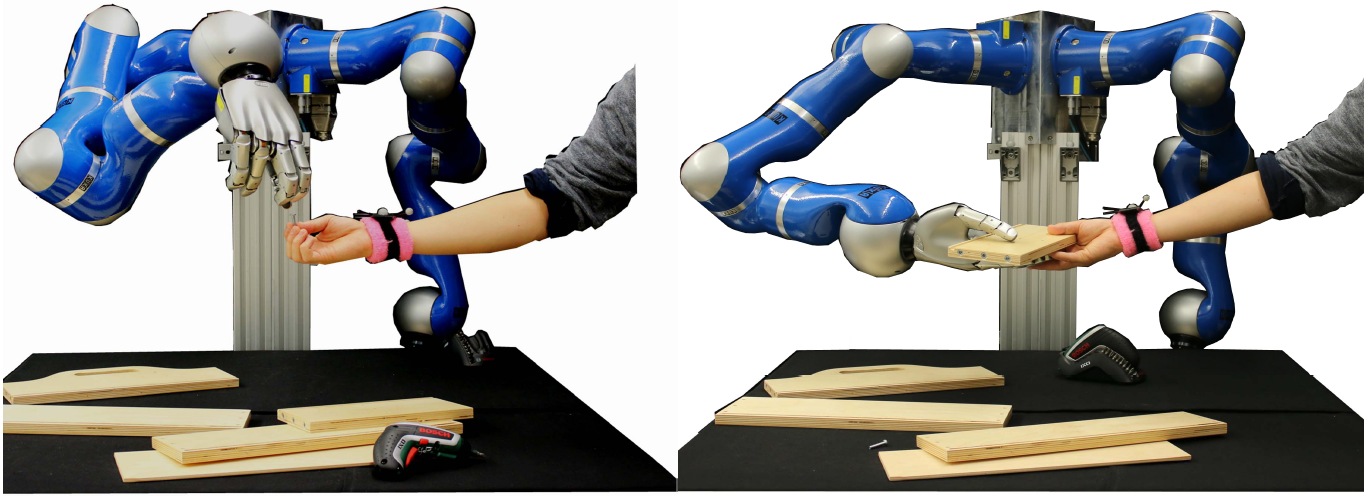
\includegraphics[width=3.5in]{figs/example.PNG}}
\caption{Situation where a robot anticipates that the worker will need a wooden plank and hands it over to him \cite{Maeda2016}}
\label{example}
\end{figure}

The remainder of the document is organized into four chapters. Chapter \ref{chapter:collaborative_robotics} describes background concepts about collaborative robotics, including safety in HRC. Chapter \ref{chapter:data_sources} reviews the data sources and sensors used in previous work on Action Anticipation. Chapter \ref{chapter:methods} contains a review of previous work on Action Anticipation in HRC, focusing on the methods. Chapter \ref{chapter:conclusion} concludes the document by stating the main points derived from this study.

\section{Collaborative Robotics}
\label{chapter:collaborative_robotics}

Human-robot collaboration (HRC) consists of robots and humans working in the same workspace towards a common goal. Classical industrial robots are usually automated to perform repetitive tasks that require high physical strength. On the other hand, tasks that require cognitive knowledge, flexibility, and precision are better suited for humans, even if they are physically weaker. HRC aims to take advantage of both of their strengths and complement each others’ weaknesses to increase manufacturing efficiency.

In an HRC scenario, robots need to be different from the traditional ones, given that they will work in the same workspace as humans. According to \textcite{Castro2021}, \textquote{Collaborative robots need to be endowed with a set of abilities that enable them to act in close contact with humans, such as sensing, reasoning, and learning. In turn, the human must be placed at the centre of a careful design where safety aspects and intuitive physical interaction need to be addressed as well.}. In \cite{CobotsWW}, it is stated that nowadays, collaborative robots are developed to be compact, easy to install and program, flexible, mobile, consistent and precise. Additionally, they positively impact employees since they are responsible for monotonous and dangerous actions and reduce the production cost for the company.

\subsection{Safety}

Safety is one of the most critical topics in collaborative robotics and the first step toward establishing a collaborative environment. According to \cite{CobotsWW}, collaborative robots (or cobots) are able to safely work with people because they have sensitive sensors that can detect the human interrupting them, causing them to stop their actions, while traditional robots would potentially injure the worker. However, given that there are tasks that require the robot to move very close to the worker, some norms were implemented: ISO 10218-1 and 10218-2. From these two standards, \textcite{Castro2021} and \textcite{Villani2018} describe the four criteria from which at least one must be met as:

\begin{enumerate}
  \item \textbf{Safety-rated monitored stop}: when a human enters the cobot’s workspace, it completely stops;
  \item \textbf{Hand guiding}: when an operator manually moves the cobot, it is compliant;
  \item \textbf{Speed and separation monitoring}: as the human moves closer to the cobot, it becomes gradually slower;
  \item \textbf{Power and force limiting}: the cobot has its operation restricted in terms of force and torque.
\end{enumerate}

\begin{figure}[htbp]
\centerline{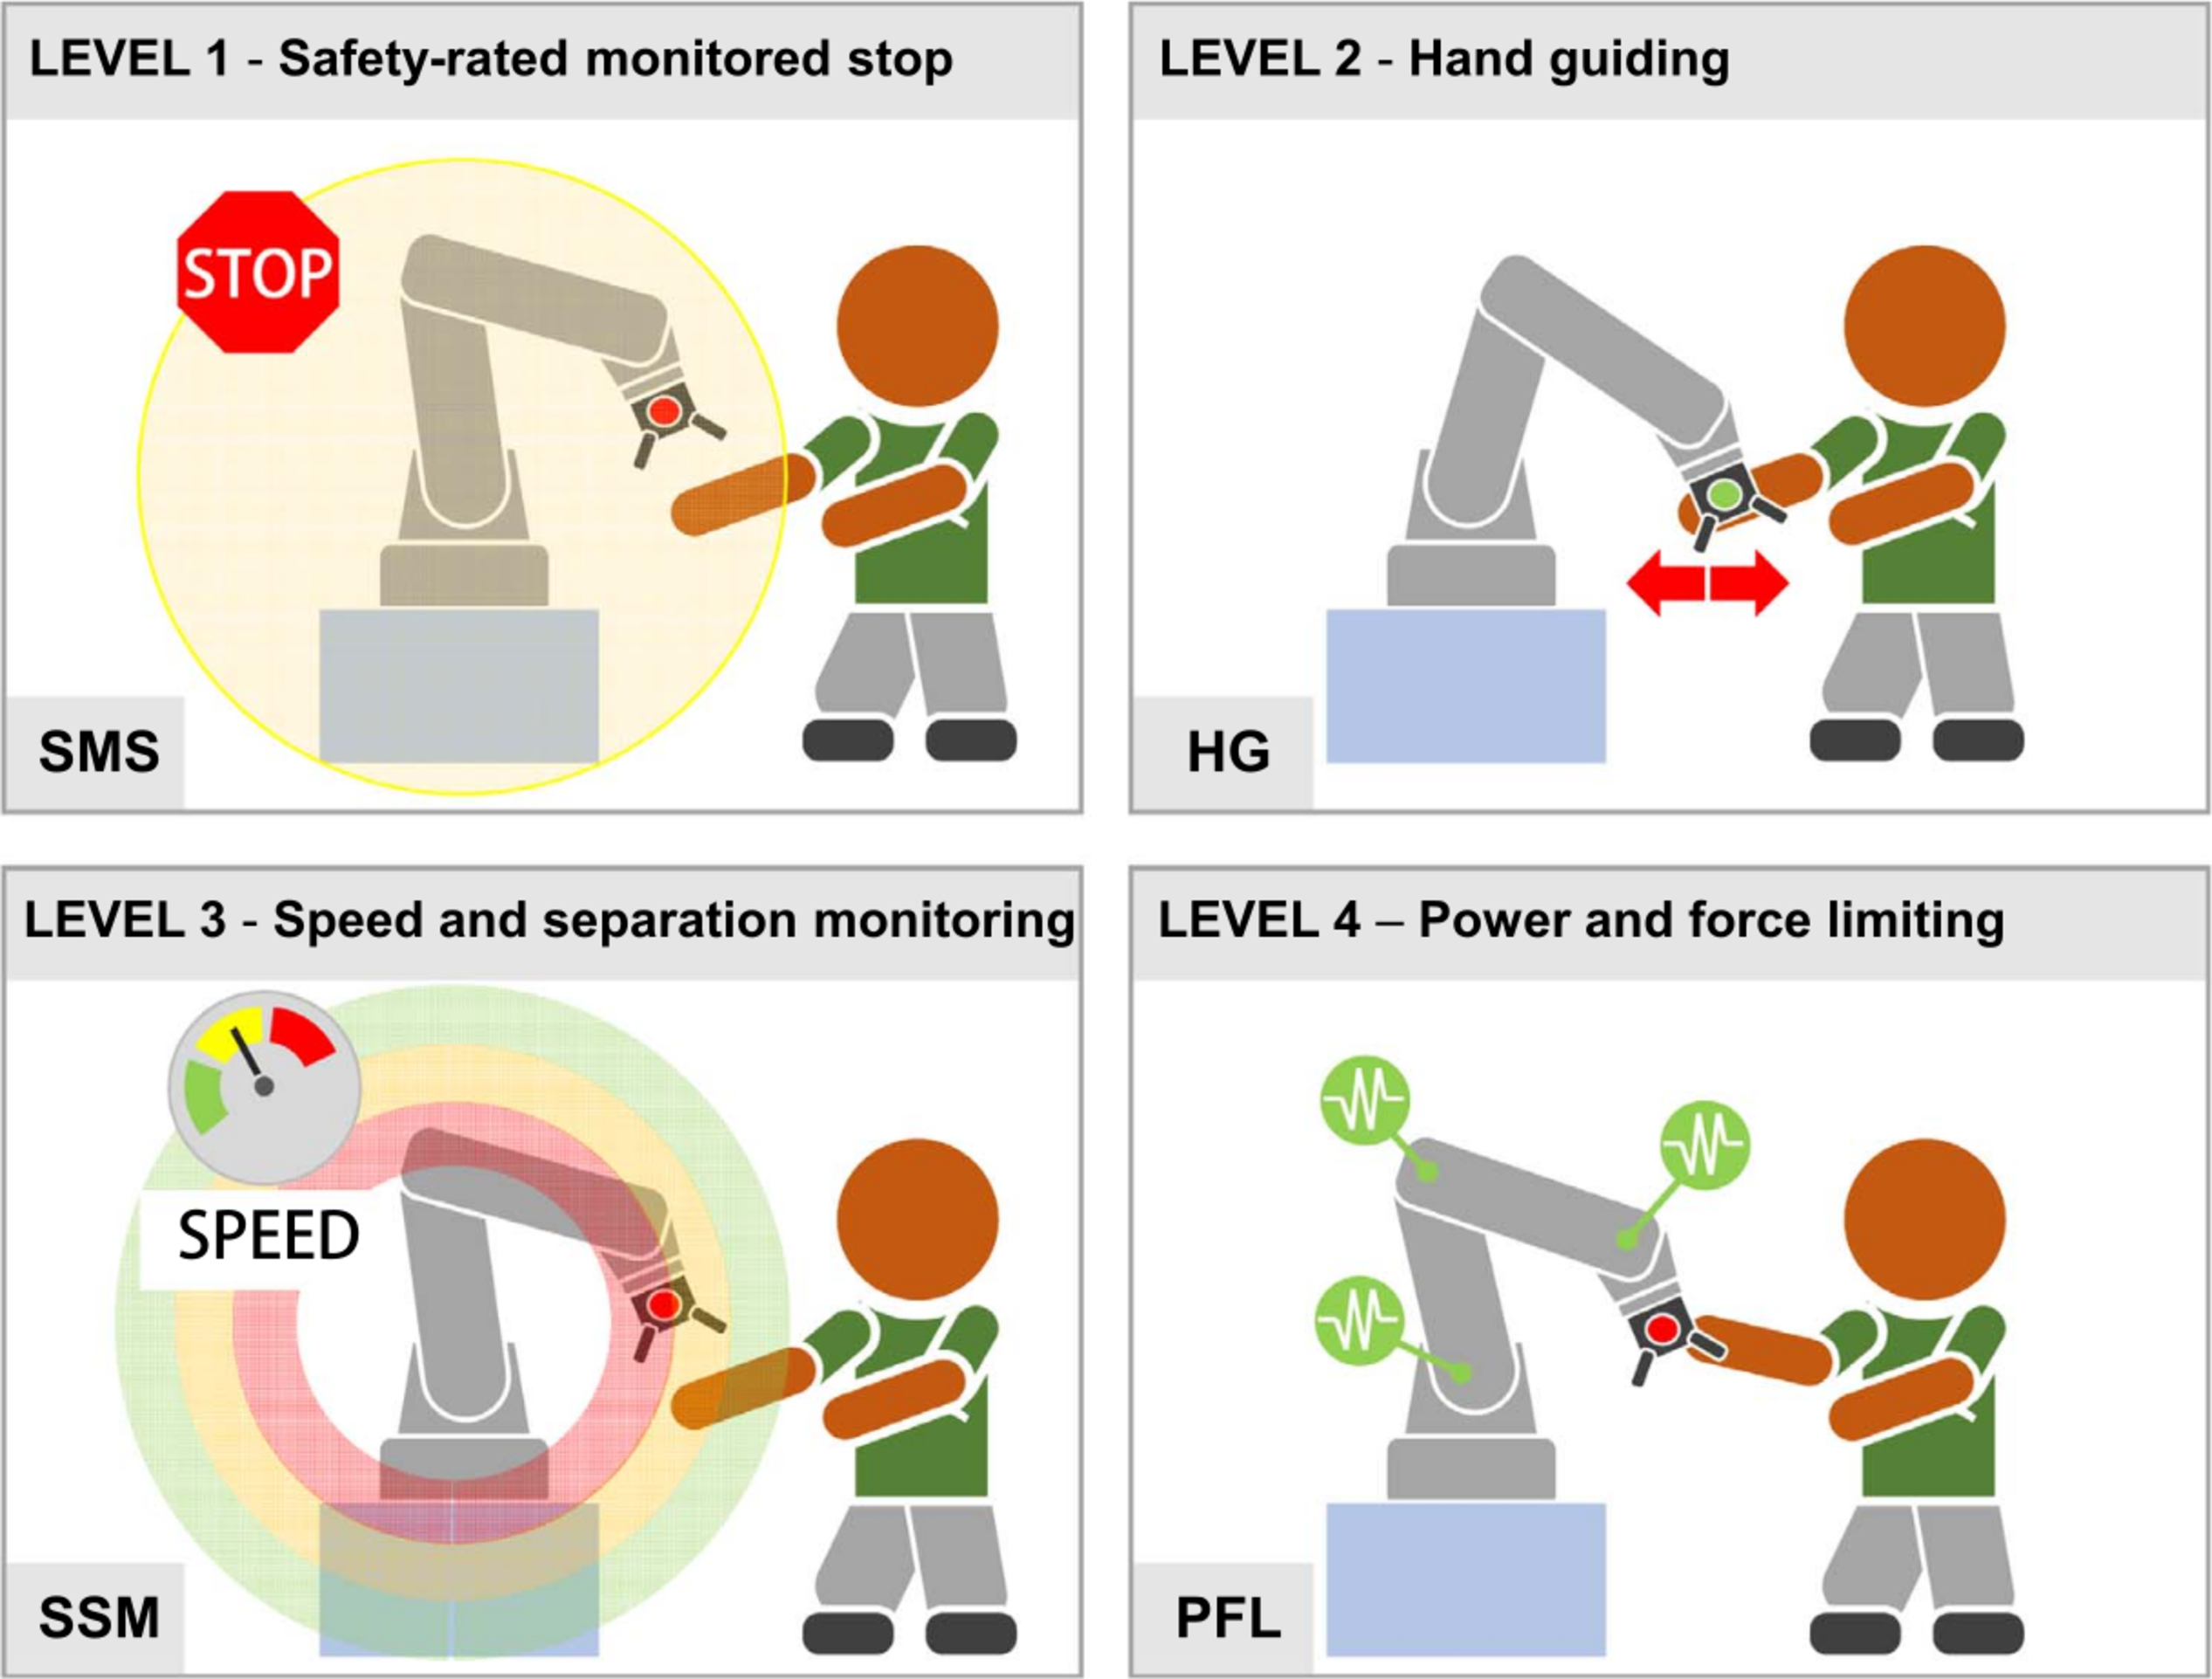
\includegraphics[width=3.5in]{figs/iso.png}}
\caption[The four collaborative operative modes identified by robot safety standards ISO modes 10218-1/2]{The four collaborative operative modes identified by robot safety standards ISO modes 10218-1/2 \cite{Villani2018}}
\label{isonorms}
\end{figure}

\section{Data Sources and Sensors}
\label{chapter:data_sources}

This section covers which data is generally used in human action anticipation and which sensors can be used to capture that data from the environment. Humans and robots can communicate through several methods, which can be direct such as using a console or a remote, or indirect, resulting from data captured from sensors. Indirect communication can be further divided into methods that work in a more active way, such as voice commands, and those that work passively. In action anticipation, passive methods are used because the user should not need to do anything for the robot to act, the robot must be able to understand the worker’s body language, such as his involuntary pose, gestures or gaze. Based on \cite{Castro2021, Mukherjee2022, Semeraro2023}, the main kinds of data in indirect and passive communication can be seen in the diagram in Fig.~\ref{interaction} and can be described as follows:

\begin{figure}[htbp]
\centerline{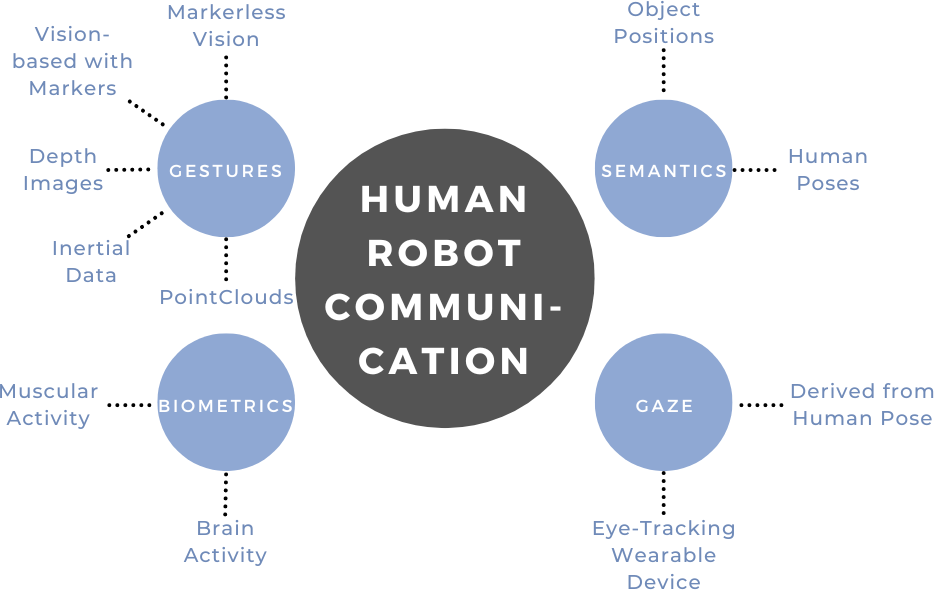
\includegraphics[width=3.5in]{figs/Action Anticipation methods.png}}
\caption{Data sources common in action anticipation}
\label{interaction}
\end{figure}

\begin{itemize}
\item \textbf{Gestures}: these are one of the main ways humans communicate, whether through simple movements or formal sign language. In the literature about HRC, gestures can also commonly be found since they have the advantage of resisting ambient noise. Usually, gestures are captured with vision-based methods with either an RGB or RGB-D camera, so there is no need for unnatural movements. With vision, it is possible to include markers, but these may lead to occlusions and hinder the worker’s movements. Consequently, there is also work in the literature that uses markerless vision to allow more unrestricted movements. Another way to capture the movements of the human worker would be to use wearable inertial sensors, which contain accelerometers and gyroscopes, but, once again, wearables can hinder the worker’s movements. Finally, capturing point clouds using a LIDAR presents another possibility of capturing gestures without restricting the worker’s motion.

\item \textbf{Semantics}: semantic information about the objects can also help the global workflow. Human actions can be represented semantically by obtaining the poses of the human as a specific set of limbs, even if only partially. During action prediction, this, coupled with the object positions, can be used to know which objects the worker can interact with. Having semantic information about the pose of the human body also helps in the path-planning phase of the robot since it can use this information to avoid the worker and prevent collisions.

\item \textbf{Gaze}: this can be used to determine where the user’s attention resides, giving a considerable amount of information that can trigger some action. There are two options to obtain the user’s gaze. Wearable sensors can provide better results but are expensive and intrusive. On the other hand, algorithms that detect head pose and assume the gaze from it can also be used, which is a cheaper and non-intrusive solution.

\item \textbf{Biometrics}: Electromyography (EMG) sensors can measure electrical signals generated by muscle contractions, while electroencephalography (EEG) sensors are commonly used in brain-computer interfaces (BCIs). %\textcolor{blue}{And why not heart beat, breath, ...?}

\end{itemize}

Regarding the sensors used to capture the raw data, most literature suggests using an RGB camera. However, the captured images may be used in the following different ways:

\begin{itemize}
\item directly used as input to models which can extract features from the images;

\item used as input to frameworks that receive an image, process it, and return the key points, such as the skeleton joints of the person in the image; these key points can also then be used to assume the gaze of the human in the image such as in \textcite{Canuto2021} where the authors used OpenPose\cite{Cao2021,Simon2017,Cao2018,Wei2016}\footnote{OpenPose documentation:

\url{https://cmu-perceptual-computing-lab.github.io/openpose}}, an open-source project that aims to detect key points in the human body, face, hands, and feet from images as shown in Fig.~\ref{openpose}, to obtain not only the skeleton joints but also the worker’s gaze;

\item used to process the optical flow \cite{Gammulle2019, Wu2021, Rodriguez2019, Furnari2021};

\item if the human was wearing markers, the image can be used to obtain the positions of the markers obtaining gestures from the sequence of those positions \cite{Maeda2016};
\end{itemize}

\begin{figure}[htbp]
\centerline{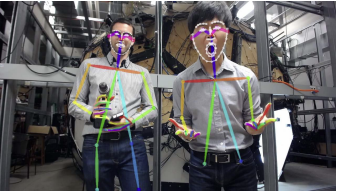
\includegraphics[width=3.5in]{figs/openpose.jpeg}}
\caption[OpenPose Example]{OpenPose Example \cite{Cao2021}}
\label{openpose}
\end{figure}

Besides RBG cameras, some works, such as the one described in \textcite{Moutinho2023}, indicate the use of an RGB-D camera to capture both the color and the depth images, which contain the gestures and pose of the worker. Other than cameras, in \textcite{Tortora2019} IMU and EMG data was used as input to capture the gestures and anticipate the worker’s action. When it comes to obtaining the worker’s gaze, it is possible to do so from the RGB images, as mentioned before, but it is also possible to use wearable sensors to capture it, such as in \textcite{Schydlo2018}.

\section{Methods}
\label{chapter:methods}

After exploring which kinds of data are usually captured and provided to an algorithm, this section covers algorithmic solutions, particularly those that make use of machine learning methodologies.

%starting by those that are only about predicting the action of the human worker and then those that go a step further and reference how to go from a prediction to the action that the robot must execute as a response.

Artificial intelligence has significantly evolved in the last few years. With the increase of computational power, machine learning, a subset of AI, has become an increasingly promising method to deal with complex and multidimensional data like images and text, heavily contributing to areas such as visual perception and speech recognition. Machine learning’s ability to learn from data with minimal human intervention and make predictions or decisions from new data it has never seen before makes it a prime candidate to solve many problems in robotics and, in particular, action anticipation in collaborative environments. The most common strategies in this field are Supervised Learning, Unsupervised Learning, and Reinforcement Learning.

\begin{itemize}
\item \textbf{Supervised Learning}: the models are trained using a dataset of labeled data. According to \textcite{Sarker2021}, these models must generalize the knowledge from the dataset’s input-output pairs to correctly deal with a new input they have never seen before. The models from this group are further divided into classification, where the new input is assigned a discrete output class, and Regression, where it is returned a real number from the continuous output space. Currently, RNNs and CNNs are two of the most common classification approaches.

\item \textbf{Unsupervised Learning}: the datasets involved have no labels. According to \textcite{Sarker2021}, these algorithms aim to find patterns and structure in the data. This makes them valuable in tasks such as clustering based on common characteristics, density estimation, identifying anomalies and outliers, dimensionality reduction, feature learning and finding association rules.

\item \textbf{Reinforcement Learning}: machine learning approach different from the previous ones because it does not need a dataset. According to \textcite{Alom2019}, the agent learns how to act in an unknown environment by interacting with it. After the agent’s action, the environment returns an observation and a certain reward to the agent, depending on the quality of the action. The agent uses the reward to update its internal model named policy improving its future performance and the cycle repeats. This type of learning by trial and error has a certain resemblance to how humans gain knowledge, and it is useful when there is a need for an agent to make decisions in an environment that has considerable complexity, such as controlling a robot or playing a game.
\end{itemize}

\begin{figure}[htbp]
\centerline{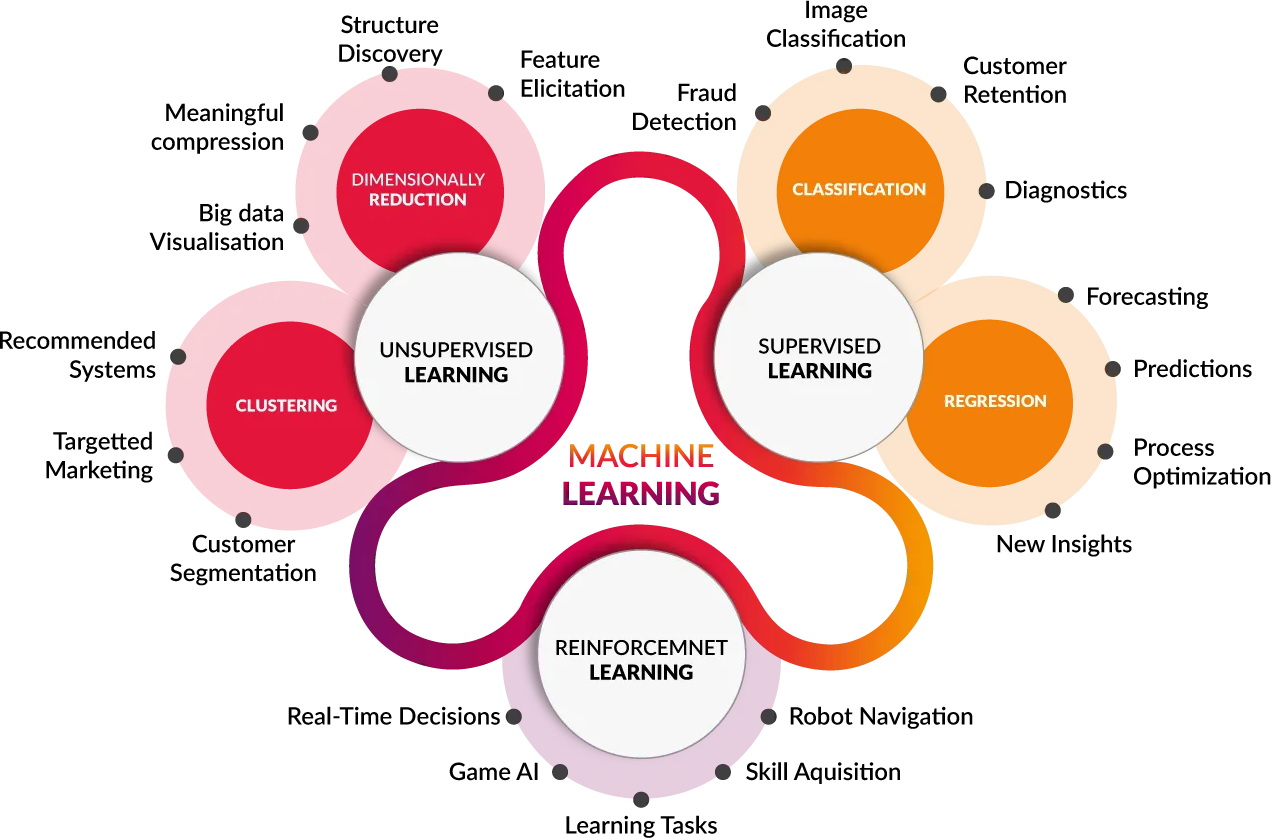
\includegraphics[width=3.5in]{figs/ml_types2.png}}
\caption{Use cases of the different types of machine learning \cite{ml_types}}
\label{ml_types}
\end{figure}

The next subsections mainly contain possible solutions present in previous work, which are described in reasonable detail since they vary not only in algorithms but also in the input data.

\subsection{Predictive Modeling Techniques}

Predicting the next action of the worker can be represented as a classification problem since it is possible to use a sequence of images that must be classified as a particular future action class. Using Fig.~\ref{superviseddiagram} as an example, the high-five action should be predicted before the frames that contain it are captured.

\begin{figure}[htbp]
\centerline{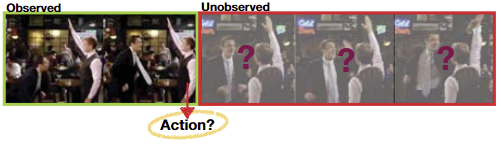
\includegraphics[width=3.5in]{figs/superviseddiagram.PNG}}
\caption[Action Anticipation using Supervised Learning diagram]{Action anticipation using supervised learning diagram \cite{Gammulle2019}}
\label{superviseddiagram}
\end{figure}

The previous work on predictive models mainly includes CNNs and RNNs, with the latter being the most common and transfer learning also being a frequent technique.

\begin{itemize}
\item \textbf{Recurrent Neural Network (RNN)}: type of neural network where the output of each time step is fed back into the input at the next time step, allowing the network to remember and incorporate information from previous time steps into its processing of current and future data. This characteristic makes RNNs particularly well-suited to processing sequential data, such as text, speech, or time series data which require context or temporal dependencies. In particular, according to \cite{lstm_advantages}, Long Short-Term Memory (LSTM) is an RNN with a more complex architecture that gives it an improved ability to backpropagate the error, making it better to train a model that classifies sequences with several time steps.

\item \textbf{Convolutional Neural Network (CNN)}: type of neural network made up of several convolutional layers which apply a sliding filter over the input reducing its dimension and obtaining its features. Typically, these layers are followed by one or more fully connected layers that perform the prediction using the mentioned features. This architecture makes CNNs an excellent choice to deal with data in a matrix structure such as an image because this input is too massive for manual feature engineering.

\item \textbf{Transfer Learning}: technique that makes use of a trained external model. Depending on the goal of its use, these models can be entirely or partially used; optionally, they can also be trained partially or fully. A common use case for this technique in supervised learning is when a small dataset of images is used to obtain a classifier. A standard model cannot generalize from that reduced amount of data. In this case, a model such as VGG-16 and ResNet-50 can be used partially to extract the features with one or more fully connected layers in the end, to perform the desired classification from those features.
\end{itemize}

% LSTM only examples
In \textcite{Furnari2021}, the authors aimed to predict the subsequent actions that someone wearing a camera would perform and the objects he would interact with. They used three datasets containing RBG frames from which they derived the optical flow and the objects in the environment. This data is then passed on to a Rolling-Unrolling LSTM. The Rolling LSTM (R-LSTM) is a network that continuously encodes the received observations and keeps an updated summary of the past. When it is time to make predictions about future actions, the Unrolling LSTM (U-LSTM) is used with its hidden and cell states equal to the current ones of the R-LSTM.

In \textcite{Schydlo2018}, the authors used an encoder-decoder recurrent neural network topology to predict human actions and intent where the encoder and the decoder are both LSTM cells. At each step, the decoder returns a discrete distribution of the possible actions making this algorithm able to consider multiple action sequences, which are then subject to a pruning method that reduces them to obtain the right action finally. In their work, these algorithms were tested in two different datasets, one containing RGB images with optical markers and gaze information from wearable sensors and another with RGB-D images.

% ResNet-34 + LSTM
In \textcite{Moutinho2023}, the authors aimed to increase the natural collaboration between the robot and the human in an assembly station by interpreting implicit communication cues. The data related to the environment was captured using an RGB-D camera. This data was then passed on to a ResNet-34, a pre-trained neural network that extracted the features from the images. These features are used as the input to an LSTM to perform human action recognition.

% ResNet-50 + LSTM
In \textcite{Gammulle2019}, the authors aimed to predict future frames while at the same time predicting the following action. In their implementation, they used public datasets with videos from which they obtained RGB images and optical flow streams. To consider both data sources, they also used two ResNet-50’s, which are pre-trained networks, one to get the input features from the image and another from the optical flow, and 2 LSTMs to take into account both sequences of inputs. Then the two results are merged into a final classification. They also used two Generative Adversarial Networks (GAN) to generate the subsequent frames, but this is different from the focus of the analysis.

%% VGG-16 + TTM
In \textcite{Wang2021}, the authors used video datasets to train a model that would predict a future action from the observed frames. They used three pre-trained neural networks in their work: VGG-16, TS, and ConvNet, to extract features from the images. Then these features were aggregated using a Temporal Transformer module (TTM), and finally, a progressive prediction module (PPM) would anticipate the worker’s future action. This article also addresses the issue of specifying what the algorithm should consider as an action. Although most of the literature often implies that the last frames captured by the camera are considered an action, given that those are the frames that contain the last action made by the user, the authors of this article go into greater detail. They tested and evaluated how many frames should be considered as the last action to obtain the best results using a metric from \textcite{Geest2016} named per-frame calibrated average precision (cAP) calculated with \eqref{eq}. In \cite{Wang2021} it is defined with
\begin{equation}
cAP=\frac{\sum_k cPrec(k) * I(k)}{P},
\label{eq}
\end{equation}
\textquote{... where  calibrated  precision $cPrec=\frac{TP}{TP+FP/w}$, $I(k)$ is an indicator function that is equal to 1 if the cut-off frame k is a true positive, $P$ denotes the total number of true positives, and $w$ is the ratio between negative and positive frames. The mean cAP over all classes is reported for final performance.}.

%% CNN
In \textcite{Rodriguez2019}, the authors aimed to predict the following action by first predicting the following motion images. They used datasets containing videos and then processed them to obtain motion images. These motion images become the input of a convolutional autoencoder network that generates the following motion images. These images are then passed to a CNN that processes them and makes action predictions for the future. The final action prediction is obtained from the results of the previous network and those of a second CNN, which analyzes the original RGB images.

%% architecture with TSN
In \textcite{Wu2021}, the author’s goal was to predict the following action someone wearing a camera would perform after some time. Initially, the optical flow was obtained from the captured images, and both were used as input to the model. The model is comprised of a Temporal Segment Networks (TSN), a CNN, and an LSTM to predict the future frame features and then use them to perform the required classification.

\subsection{From Prediction to Planning}

After predicting the next action of the worker, the robot must execute some action as a response to complete the anticipation process. This subsection contains articles that go beyond the predictive model and have relevant details for the integration of the model in a robot controller.

In \textcite{Canuto2021}, the authors aimed to predict the following action using an LSTM, one of the most common RNNs. In their work, they used a dataset captured with an RGB camera. From these images, they obtained the objects in the environment, the human skeleton joints extracted over time using OpenPose, and the gaze derived from the joints. Then the three data sources were given to the LSTM as input to perform the desired classification. In this process, the authors use an adaptive threshold on the uncertainty of the recurrent neural network, which makes the model need a certain level of certainty to classify the action as a particular class. This creates a more robust solution since a standard supervised learning algorithm would predict the class with the highest probability even if the model has low certainty about every category.

% Look-up table
In \textcite{Maeda2016}, the authors aimed to reduce the delay in the robot’s response by anticipating the human worker and providing a screw or a plate accordingly. They captured the environment using an RGB camera and tracked the hand using optical markers. Then they predicted the following human action using a look-up table containing different orders for assembly actions. With the nearest neighbor algorithm, the actions of the human would be matched with a particular order. The limitation of this method is that all possible sequences need to be on the table because if they are not there, then the robot will match with a different order which may be undesirable. If the robot eventually notices that it did the wrong action, it would then follow a hard-coded contingency trajectory to return to the pre-grasping position. When performing a handover action, the previously captured data is used to generate possible trajectories, and this is given to the feedback controller as a reference.

% LSTM + CNN
In \textcite{Zhang2022}, the authors aimed to predict the intention of the human worker to provide him with the required piece. To achieve this, they used an RGB camera to capture the data from the environment. Then the images are given to a convLSTM framework where the CNN part is in charge of extracting features from the input images, and these features are then passed on to the LSTM to predict the intention. This article also tackles the issue of having several possible assembly orders. It solves it by creating a phase at the beginning of the collaboration in which the robot learns the assembly actions and their order from a demonstration. After the prediction of the intention of the worker, the robot proceeds to fetch the required piece. It uses a CNN to recognize said piece and ROS Open Motion Planning Library (OMPL) to handle the trajectory planning jobs. In terms of safety, the authors defined speed limits for the robot and ensured that the robot would avoid the workspace of the human. Then when it needs to move closer to the user, its speed is reduced to guarantee the user’s safety.

In \textcite{Huang2016}, the goal of the authors is to make the robot use the anticipated actions of the worker to decide its tasks. It monitors the worker’s gaze using a wearable device and uses it to predict his intent using SVM. After predicting it, the robot uses an anticipatory motion planner named \textquote{MoveIt!} to plan its motion according to a certain confidence threshold. This means that while it is unsure of what the human wants, the robot starts to move toward the item it thinks he wants but only really moves completely when it surpasses the threshold.

\section{Conclusion}
\label{chapter:conclusion}

This document presented a review of the problem of anticipating human actions in collaborative environments. Although initially, it was also referred that an end-to-end learning technique could be used, the articles found all pointed towards separately developed modules. Looking at previous work found in the literature, there is a clear predominance of perception using RGB cameras with different ways of preprocessing the captured images. When it comes to the methods, machine learning and, in particular, supervised learning techniques are predominant, given that most work nowadays takes advantage of the progress made in that field. With the continuous evolution of machine learning, it is expected that the algorithms related to the topic in this paper also evolve and, consequently, give rise to even better solutions.

In summary, the results of this study demonstrate that Action Anticipation is still a relatively new concept, but it has much potential to increase the efficiency and safety of collaborative tasks, revolutionizing the world of human-robot collaboration.

\section{References}
%Print all used references
\begingroup
\renewcommand{\bibfont}{\footnotesize}

%Redefine References name
\defbibheading{bibliography}[]{
	\chapter{#1}
}
%\SingleSpacing
\setlength\bibitemsep{8pt}
\printbibliography[heading=bibliography]
\endgroup

\end{document}
